%%==================================================
%% chapter01.tex for SJTU Master Thesis
%% based on CASthesis
%% modified by wei.jianwen@gmail.com
%% version: 0.3a
%% Encoding: UTF-8
%% last update: Dec 5th, 2010
%%==================================================

%\bibliographystyle{sjtu2} %[此处用于每章都生产参考文献]
\chapter{背景介绍}
\label{chap:background}


\section{移动无线网络}
\label{sec:mobile}

\subsection{高速移动网络}
\label{sec:gsmr}


\subsection{无线局域网络}
\label{sec:80211n}

Wireless local area networking has experienced tremendous growth in the last ten years
with the proliferation of IEEE 802.11 devices. Its beginnings date back to Hertz’s discovery
of radio waves in 1888, followed by Marconi’s initial experimentation with
transmission and reception of radio waves over long distances in 1894. In the following
century, radio communication and radar proved to be invaluable to the military, which
included the development of spread spectrum technology. The first packet-based wireless
network, ALOHANET, was created by researchers at the University of Hawaii in
1971. Seven computers were deployed over four islands communicating with a central
computer in a bi-directional star topology.

\url{http://www.pewinternet.org/default.aspx}

A milestone event for commercial wireless local area networks (WLANs) came
about in 1985 when the United States Federal Communications Commission (FCC)
allowed the use of the experimental industrial, scientific, and medical (ISM) radio bands
for the commercial application of spread spectrum technology. Several generations of
proprietary WLAN devices were developed to use these bands, including WaveLAN by
Bell Labs. These initial systems were expensive and deployment was only feasible when
running cable was difficult.

Advances in semiconductor technology and WLAN standardization with IEEE 802.11
led to a dramatic reduction in cost and the increased adoption of WLAN technology.
With the increasing commercial interest, the Wi-Fi Alliance (WFA) was formed in
1999 to certify inter operability between IEEE 802.11 devices from different manufacturers
through rigorous testing. Since 2000, shipments of Wi-Fi certified integrated
circuits (IC) reached 200 million per year in 2006 (ABIresearch, 2007). Shipments are
expected to exceed a billion units per year by 2012 (ABIresearch, 2007), as illustrated in
Figure 1.1.

Such large and sustained growth is due to the benefits WLANs offer over wired
networking. In existing homes or enterprizes, deploying cables for network access may
involve tearing up walls, floors, or ceilings, which is both inconvenient and costly.
In contrast, providing wireless network connectivity in these environments is often as
simple as installing a single wireless access point. Perhaps more importantly though, the
proliferation of laptops and hand held devices has meant that people desire connectivity
wherever they are located, not just where the network connection is located. Network
connectivity in a conference room or while seated on the sofa in the living room are just
two examples of the flexibility afforded by WLANs.

\begin{figure}[!htp]
\centering
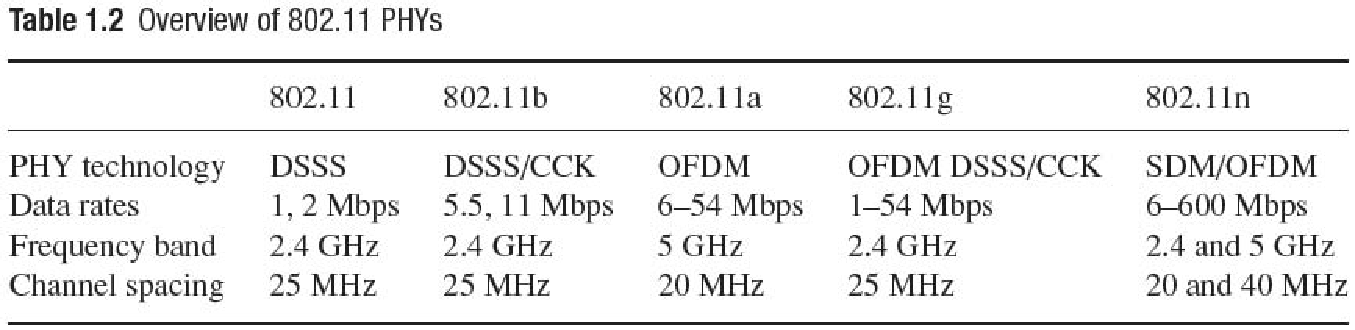
\includegraphics[width=0.5\textwidth]{chap1/change.pdf}
\bicaption[fig:change]{802.11n网络特性}{802.11n网络特性}{Fig}{Feather of 802.11n Networks}
\end{figure}

\begin{figure}[!htp]
\centering
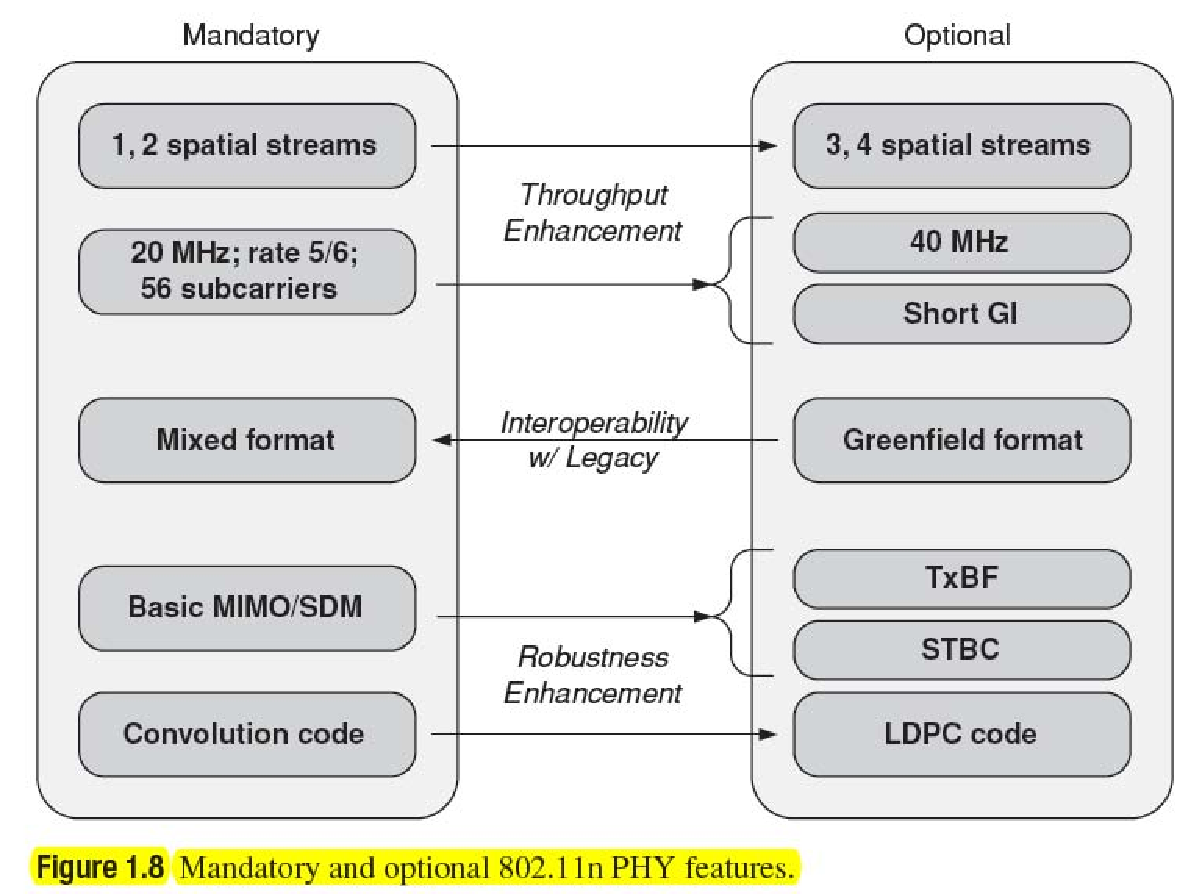
\includegraphics[width=0.5\textwidth]{chap1/PHYfeather.pdf}
\bicaption[fig:phyfeather]{802.11n网络PHY特性}{802.11n网络PHY特性}{Fig}{Feather of 802.11n Networks}
\end{figure}

\begin{figure}[!htp]
\centering
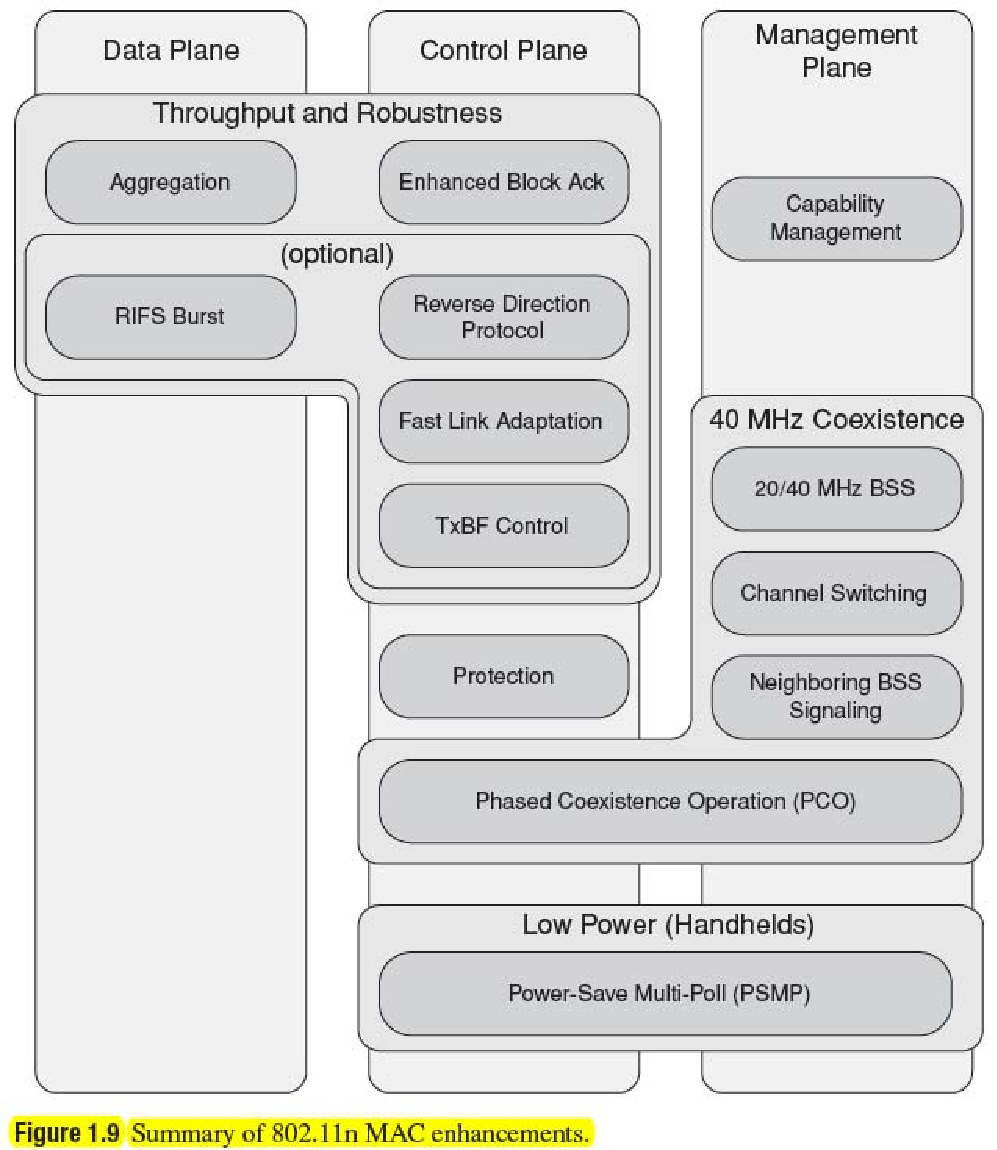
\includegraphics[width=0.5\textwidth]{chap1/MACfeather.pdf}
\bicaption[fig:macfeather]{802.11n网络MAC特性}{802.11n网络MAC特性}{Fig}{Feather of 802.11n Networks}
\end{figure}

This comprehensive overview describes the underlying principles, implementation details, and key enhancing
features of 802.11n. For many of these features, the authors outline the motivation and
history behind their adoption into the standard. A detailed discussion of the key throughput,
robustness, and reliability enhancing features (such as MIMO, 40 MHz channels,
and packet aggregation) is given, in addition to a clear summary of the issues surrounding
legacy inter operability and coexistence. The key features of all the proposals were similar, including spatial division multiplexing and 40 MHz channels for increased data rate, and frame aggregation for improved
MAC efficiency.
	
\subsubsection{Network Structure}

1.3 Environments and applications for 802.11n

The basic service set (BSS) is the basic building block of an 802.11 LAN. Stations that
remain within a certain coverage area and form some sort of association form a BSS. The
most basic form of association is where stations communicate directly with one another
in an ad-hoc network, referred to as an independent BSS or IBSS. This is illustrated as
BSS 1 in Figure 1.4.

\begin{itemize}
  \item Mesh
  \item Ad-hoc
\end{itemize}

\subsubsection{Physical Layer Technology}
\begin{itemize}
  \item Spatial Diversity
  \item Channel Bonding
\end{itemize}

\subsubsection{Medium Access Control Layer Enhancements}
\begin{itemize}
  \item Frame Aggregation
  \item Streamlined ACK
\end{itemize}

\subsubsection{Wireless Driver and Extension}
\begin{itemize}
  \item ieee80211
  \item ath9k
  \item iw
\end{itemize}

\subsubsection{Rate Adaption}

  1. sample
    \begin{enumerate}
      \item The rate chosen by sample did not alter to match changes in the radio
	    environment.
      \item Higher throughput (between two nodes) could often be achieved by fixing
	    the bitrate of both nodes to some value.
      \item After a long period of operation, "sample" appeared to be stuck in a low
	    data rate, and would not move to a higher data rate.
    \end{enumerate}

  2. minstrel
    EWMA calculations are used to process the success history of each rate. On
	completion of the calculation, a decision is made as to the rate which has the
	best throughput, second best throughput, and highest probability of success.
	This data is used for populating the retry chain during the next 100 ms.

    The EWMA calculation is carried out 10 times a second, and is run for each
	rate. This calculation has a smoothing effect, so that new results have a
	reasonable (but not large) influence on the selected rate. However, with time,
	a series of new results in some particular direction will predominate.

    Minstrel spends a particular percentage of frames, doing "look
	around" i.e. randomly trying other rates, to gather statistics. The percentage
	of "look around" frames, is set at boot time via the module parameter
	"ath\_look-around\_rate" and defaults to $10\%$. The distribution of look-around
	frames is also randomized somewhat to avoid any potential "strobing" of
	look-around between similar nodes.

    The contention window size does vary with traffic class. For example, video
	and voice have a contention window min of 3 and 2 microseconds
	respectively. Currently, minstrel does not check traffic class.	Calculating the throughput based on traffic class and bit rate and variable
	packet size will significantly complicate the code and require many more
	sample packets. More sample packets will lower the throughput achieved. Thus,
	our view is that for this release, we should take a simple (but reasonable)
	approach that works stably and gives good throughput.

  3. ath9k

\begin{table}[!htp]
\renewcommand{\arraystretch}{1}
\bicaption[tab:mcs]{802.11n网络MCS索引}{802.11n网络MCS索引}{Table}{MCS index of 802.11n}
\centering
\begin{threeparttable}[b]
\begin{tabular}{cccccc}
\hline
  \multirow{2}{*}{MCS} & \multirow{2}{*}{Modulation} & \multirow{2}{*}{Code Rate} & \multirow{2}{*}{Rate (Mbps)} & \multicolumn{2}{c}{Sensitivity (dBm)} \\
\cline{5-6}
  & & & & Typical & Max \\
\hline
  0 & BPSK & 1/2 & 6.5 & -94 & -85 \\
%\cline{2}
  1 & QPSK & 1/2 & 13.0 & -92 & -82 \\
%\cline{2}
  2 & QPSK & 3/4 & 19.5 & -90 & -80 \\
%\cline{2}
  3 & 16 QAM & 1/2 & 26.0 & -87 & -77 \\
%\cline{2}
  4 & 16 QAM & 3/4 & 39.0 & -84 & -73 \\
%\cline{2}
  5 & 64 QAM & 2/3 & 52.0 & -79 & -69 \\
%\cline{2}
  6 & 64 QAM & 3/4 & 58.5 & -78 & -68 \\
%\cline{2}
  7 & 64 QAM & 5/6 & 65.0 & -76 & -67 \\
\hline
\end{tabular}
\end{threeparttable}
\end{table}

%\begin{table}[!htp]
%\renewcommand{\arraystretch}{1}
%\bicaption[tab:mcs]{802.11n网络MCS索引}{802.11n网络MCS索引}{Table}{MCS index of 802.11n}
%\centering
%\begin{threeparttable}[b]
%\begin{tabular}{c|c|c|ccc}
%\hline
%  Channel & MCS & Rate(Mbps) & $\beta_-$ & $\beta_0$ & $\beta_+$ \\
%\hline
%  \multirow{8}{*}{HT20/LGI} & 0 &  6.5 & -70 & -65 & -60 \\
%\cline{2}
%                            & 1 & 13.0 & -70 & -65 & -60 \\
%\cline{2}
%                            & 2 & 13.0 & -70 & -65 & -60 \\
%\cline{2}
%                            & 3 & 13.0 & -70 & -65 & -60 \\
%\cline{2}
%                            & 4 & 13.0 & -70 & -65 & -60 \\
%\cline{2}
%                            & 5 & 13.0 & -70 & -65 & -60 \\
%\cline{2}
%                            & 6 & 13.0 & -70 & -65 & -60 \\
%\cline{2}
%                            & 7 & 13.0 & -70 & -65 & -60 \\
%\hline
%  \multirow{8}{*}{HT20/SGI} & 0 &  6.5 & -70 & -65 & -60 \\
%\cline{2}
%                            & 1 & 13.0 & -70 & -65 & -60 \\
%\cline{2}
%                            & 2 & 13.0 & -70 & -65 & -60 \\
%\cline{2}
%                            & 3 & 13.0 & -70 & -65 & -60 \\
%\cline{2}
%                            & 4 & 13.0 & -70 & -65 & -60 \\
%\cline{2}
%                            & 5 & 13.0 & -70 & -65 & -60 \\
%\cline{2}
%                            & 6 & 13.0 & -70 & -65 & -60 \\
%\cline{2}
%                            & 7 & 13.0 & -70 & -65 & -60 \\
%\hline
%\end{tabular}
%\end{threeparttable}
%\end{table}


\section{通信质量测试}
\label{sec:measure}

Calculate throughput based on the average A-MPDU length, taking into account the expected number of retransmissions and their expected length.

1. Packet Delivery Ratio: $1-\frac{Retries+Failed}{Transmitted}$

2. Frame Delivery Ratio: $1-\frac{A\text{-}MPDUs * Retries + Failed MPDUs}{A\text{-}MPDUs * Retries+1}$

3. Efficient Date Rate: $DateRate * PDR$

4. Efficient Throughput: $Throughput * PDR$

\subsection{物理层信道状态估计}
\label{sec:phy}


\subsection{链路层链路质量测试}
\label{sec:mac}
